\documentclass[11pt, a4paper]{article}
\PassOptionsToPackage{hidelinks}{hyperref}
\usepackage[utf8]{inputenc} 
\usepackage{fullpage}
\usepackage{graphicx}
\usepackage{xcolor}
\usepackage{amsmath}
\usepackage{bookmark}
\usepackage{ragged2e}
\usepackage{amsmath}
\usepackage{amsfonts}
\usepackage{array}
\usepackage{float}
\usepackage{tabularx}
\usepackage{listings}
\usepackage{hyperref}
\usepackage{array}
\renewcommand\UrlFont{\color{blue}\rmfamily}
 
% Title of your project
\title{Optimization with Genetic Algorithms}

% Name of deliverable
\newcommand{\deliverableName}{Delivery of Activity 2}

% Author
\author{Javier Novella Ruiz}

% Group number
\newcommand{\groupNumber}{17685106}

% Comment
\newcommand{\comments}{Virtual student}

% Date for title page, default is today and 
\date{\today}

\makeatletter{}

\setlength{\parindent}{0pt}

\begin{document}

\begin{titlepage}
  	\newcommand{\HRule}{\rule{\linewidth}{0.3mm}}
	\center
	%------------------------------------------------
	%	Headings
	%------------------------------------------------
	
	\textsc{\LARGE Universitat Rovira i Virgili}\\[1.5cm]
	
	\textsc{\Large \deliverableName}\\[0.5cm]
	
	\textsc{\large Neural and Evolutionary Computation}\\[0.5cm]
	
	%------------------------------------------------
	%	Title
	%------------------------------------------------
	
	\HRule\\[0.4cm]
	
	{\huge\bfseries \@title}\\[0.4cm]
	
	\HRule\\[1.5cm]
	
	%------------------------------------------------
	%	Author(s)
	%------------------------------------------------

 	{\large\sc\@author}
	
	%------------------------------------------------
	%	Date
	%------------------------------------------------
	
	\vfill\vfill
	%	{\large\@date}
    \vfill\vfill\vfill
	
	%------------------------------------------------
	%	Logo
	%------------------------------------------------
	\vfill
	
\includegraphics[width=0.3\textwidth]{./urvlogo.png}
	\vfill
\end{titlepage}


\tableofcontents

\newpage

\section{Introduction}

The Genetic Algorithms (GA) \cite{WikipediaGA} are part of what it is called Evolutionary Computation \cite{WikipediaEC}.

\vspace{1em} In evolutionary computation, an initial set of candidate solutions is generated and iteratively updated. Each 
new generation is produced by stochastically removing less desired solutions, and introducing small random changes as well 
as, depending on the method, mixing parental information.

\vspace{1em} Genetic Algorithms (GA) are metaheuristic inspired by the process of natural selection that belongs to the larger 
class of evolutionary algorithms (EA), as mentioned before. Genetic algorithms are used to generate solutions to optimization 
and search problems via biologically inspired operators such as selection, crossover, and mutation.

\vspace{1em} In this work a Genetic Algorithm has been implemented to find solutions to the Job-Shop Scheduling Problem (JSSP)
\cite{WikipediaJSSP}.

\subsection{Technology used}

The following technology has been used for the development:

\begin{itemize}
    \item Visual Studio Code v1.96.4
    \item Python v3.13.0
    \item Jupyter Notebooks with Jupyter VSCode extension v2024.11.0
\end{itemize}

\section{Technical background}

\subsection{Genetic algorithm}

Genetic Algorithms (GA) are inspired by Darwinian evolution and genetic principles. Each element in the search space \eqref{equation_1} is represented by a 
chromosome \eqref{equation_2}. The search space consists of individuals, represented as vectors of 0s and 1s, with each component being a gene.

\begin{equation}
    S = \{c \in \{0, 1\}^{m}\}
    \label{equation_1}
\end{equation}

\begin{equation}
   c \in \{0, 1\}^{m}
    \label{equation_2}
\end{equation}

The process starts with an initial population of chromosomes. The population evolves through selection, reproduction, and mutation. Natural selection favors 
individuals that are best suited for the environment, driving optimization. The fitness \eqref{equation_3} of each individual determines its ability to survive and reproduce, 
influencing the next generation in the population \eqref{equation_4}.

\begin{equation}
    F(c) \geq 0
    \label{equation_3}
\end{equation}

\begin{equation}
    P = \{c^{\mu}\}_{\mu=1,...,p} \subset S
    \label{equation_4}
\end{equation}

\subsubsection{Selection}

Selection \cite{WikipediaSelection} is the process of choosing individuals from the population based on their fitness. The better the fitness, the higher the chance of being 
selected for reproduction. This simulates natural selection, where the fittest individuals are more likely to pass on their genes to the next generation.

\vspace{1em}\textbf{Roulette wheel}

Roulette wheel selection is a probabilistic method where individuals in the population are selected based on their fitness. The selection probability is proportional to the 
fitness value, with fitter individuals having a higher chance of being selected.

\vspace{1em}\textbf{Tournament selection}

tournament selection involves selecting a subset of individuals at random and choosing the best among them to be part of the next generation. This method introduces 
competition and increases the selection pressure on fitter individuals.

\subsubsection{Crossover}

Crossover \cite{WikipediaCrossover} is the process of combining the genetic material of two parent individuals to create offspring. It involves exchanging parts of their 
chromosomes to generate new solutions. This mimics the process of sexual reproduction in nature and helps combine traits from both parents.

\vspace{1em}\textbf{One-point}

One-point crossover is a genetic algorithm technique where two parent solutions are combined to create offspring. A crossover point is selected at random, and the 
genetic material from the parents is swapped at this point to produce two new solutions.

\vspace{1em}\textbf{Uniform}

Uniform crossover, however, combines the parents by selecting genes from each parent at each position based on a probability. This results in offspring that have a more mixed 
combination of their parents' traits, maintaining diversity within the population.

\subsubsection{Mutation}

Mutation \cite{WikipediaMutation} introduces small random changes to an individual’s chromosome. It helps maintain genetic diversity within the population and prevents 
premature convergence. Mutation allows the algorithm to explore new areas of the solution space that might not be reachable through selection and crossover alone.

\vspace{1em}\textbf{One-gene}

One-gene mutation refers to altering a single gene in an individual’s chromosome. This mutation is typically performed by flipping a bit in the gene sequence 
(from 0 to 1 or vice versa), which introduces small variations in the population.

\vspace{1em}\textbf{Pobabilistic}

Probabilistic mutation, on the other hand, alters genes based on a certain probability. The probability of mutation may vary, and it is typically applied to a 
all set of genes, ensuring a controlled but diverse exploration of the solution space.

\subsection{Job-Shop Schedule Problem (JSSP)}

The Job-Shop Scheduling Problem (JSSP) involves assigning a set of jobs \(J = \{J_{1}, J_{2}, ..., J_{n}\}\) to a set of machines \(M = \{M_{1}, M_{2}, ..., M_{n}\}\) 
while respecting specific constraints. Each job consists of a sequence of operations \(O= \{O_{1}, O_{2}, ..., O_{n}\}\) that need to be processed on certain machines, 
with each operation requiring a specified amount of time. The goal is to determine an optimal schedule that minimizes the makespan, which is the total time required to 
complete all jobs, while ensuring that machine constraints and job sequences are adhered to.

\vspace{1em} Suppose also that there is some cost function \(C:X \rightarrow [0,+\infty ]\). The cost function may be interpreted as a "total processing time", and may 
have some expression in terms of times \(C_{ij}:M \times J \rightarrow [0,+\infty ]\), the cost/time for machine \(M_{i}\) to do job \(J_{j}\).

\vspace{1em} The job-shop problem is to find an assignment of jobs \(x \in X\) such that \(C(x)\) is a minimum, that is, there is no \(y \in X\) such taht \(C(x) > C(y) \).

\section{Implementation}

To implement the genetic algorithm for the Job-Shop Scheduling Problem (JSSP), a Python script in Jupyter Notebooks has been created. For better understanding of the algorithm 
developed, it is going to be broken down and explained step by step.


\subsection{Software architecture - GeneticOptimizatorJSSP class}

To develop the solution a new class has been developed GeneticOptimizatorJSSP. This class encapsulates the logic of the genetic algorithm for solving the Job-Shop 
Scheduling Problem, making the implementation modular and reusable. By organizing the methods and data within a class, the code becomes more maintainable, as the 
different components of the algorithm (population initialization, fitness evaluation, selection, crossover, and mutation) are neatly separated and can be modified 
independently. It also allows for easy instantiation and reuse of the optimization process, enabling the user to work with different sets of job data or modify 
parameters without altering the core logic. Using a class structure enhances readability, scalability, and debugging, making it more efficient to expand or adjust the 
algorithm in the future.

\subsubsection{Methods}

\begin{itemize}
    \item \_\_init\_\_(self): Initializes the class with empty job data, solution lists, and best solution placeholders.
    \item \_get\_number\_of\_machines(self, jobs): Calculates the number of machines used in the job shop based on the job data.
    \item get\_jobs(self): Returns the current job data.
    \item set\_jobs\_from\_string(self, jobs): Sets job data from a string, converting it into a list of operations and machines.
    \item set\_jobs\_from\_file(self, jobs): Sets job data from a file, reading and parsing the operations and machines.
    \item \_initialize\_population(self, population\_size): Generates an initial population of chromosomes (solutions) by creating random permutations of job operations, respecting job dependencies.
    \item \_evaluate\_fitness(self, population): Calculates the fitness of each individual in the population based on the makespan, or total processing time.
    \item \_selection(self, population, fitness, method='roulette-wheel'): Selects two parents from the population using either roulette-wheel or tournament selection methods.
    \item \_crossover(self, individual\_1, individual\_2, method='one-point'): Performs crossover on two selected individuals to produce two offspring using either uniform or one-point method.
    \item \_mutate(self, individual, method, probability=0.5): Applies mutation on an individual with a specified probability, either flipping one gene or applying probabilistic mutation.
    \item \_elitism(self, popuplation\_1, population\_1\_fitness, population\_2, number=1): Ensures the best individuals from the previous generation are retained in the new population.
    \item \_get\_best\_solution(self, population, fitness): Finds the best solution in the population by identifying the individual with the lowest makespan.
    \item run\_genetic\_algorithm(self, num\_generations, population\_size, selection\_method, crossover \_method, mutation\_method, mutation\_probability, elitism\_number): Runs the genetic algorithm for a specified number of generations, performing selection, crossover, mutation, and elitism to optimize the job-shop schedule.
\end{itemize}

\subsubsection{Attributes}

\begin{itemize}
    \item jobs: Stores the job data, which includes operations and processing times for each job.
    \item number\_of\_jobs: Holds the total number of jobs in the job-shop scheduling problem.
    \item number\_of\_machines: Stores the number of distinct machines used in the job-shop scheduling.
    \item solutions: A list that holds all the solutions (chromosomes) in the population.
    \item solutions\_fitness: Holds the fitness values (makespan values) for each solution in the population.
    \item best\_solution: Stores the best solution (chromosome) found during the genetic algorithm execution.
    \item best\_solution\_fitness: Holds the fitness (makespan) value of the best solution found.
\end{itemize}

\subsection{Loading the problem}

The problem is loaded using the methods set\_jobs\_from\_string(self, jobs), that sets job data from a string, or 
set\_jobs\_from\_file(self, jobs), that eets job data from a file. independently of the method used the expected
format of the data is a matrix \((n_{jobs} \times n_{machines})\) each element of the matrix is formed by the pair
machine number and processing time \(m_{i}, t_{i}\). Here it is an example from https://people.brunel.ac.uk/~mastjjb/jeb/orlib/files/jobshop1.txt,
specifically the Adams, Balas, and Zawack \(10 \times 10\) instance.
\[
\begin{bmatrix}
4\; 88 & 8\; 68 & 6\; 94 & 5\; 99 & 1\; 67 & 2\; 89 & 9\; 77 & 7\; 99 & 0\; 86 & 3\; 92 \\
5\; 72 & 3\; 50 & 6\; 69 & 4\; 75 & 2\; 94 & 8\; 66 & 0\; 92 & 1\; 82 & 7\; 94 & 9\; 63 \\
9\; 83 & 8\; 61 & 0\; 83 & 1\; 65 & 6\; 64 & 5\; 85 & 7\; 78 & 4\; 85 & 2\; 55 & 3\; 77 \\
7\; 94 & 2\; 68 & 1\; 61 & 4\; 99 & 3\; 54 & 6\; 75 & 5\; 66 & 0\; 76 & 9\; 63 & 8\; 67 \\
3\; 69 & 4\; 88 & 9\; 82 & 8\; 95 & 0\; 99 & 2\; 67 & 6\; 95 & 5\; 68 & 7\; 67 & 1\; 86 \\
1\; 99 & 4\; 81 & 5\; 64 & 6\; 66 & 8\; 80 & 2\; 80 & 7\; 69 & 9\; 62 & 3\; 79 & 0\; 88 \\
7\; 50 & 1\; 86 & 4\; 97 & 3\; 96 & 0\; 95 & 8\; 97 & 2\; 66 & 5\; 99 & 6\; 52 & 9\; 71 \\
4\; 98 & 6\; 73 & 3\; 82 & 2\; 51 & 1\; 71 & 5\; 94 & 7\; 85 & 0\; 62 & 8\; 95 & 9\; 79 \\
0\; 94 & 6\; 71 & 3\; 81 & 7\; 85 & 1\; 66 & 2\; 90 & 4\; 76 & 5\; 58 & 8\; 93 & 9\; 97 \\
3\; 50 & 0\; 59 & 1\; 82 & 8\; 67 & 7\; 56 & 9\; 96 & 6\; 58 & 4\; 81 & 5\; 59 & 2\; 96
\end{bmatrix}
\]

The identification of the elements from the previous input data example is shown in the following matrix.
\[
\begin{array}{r|cccccccccccccccccccc}
     & m_0 & t_0 & m_1 & t_1 & m_2 & t_2 & m_3 & t_3 & m_4 & t_4 & m_5 & t_5 & m_6 & t_6 & m_7 & t_7 & m_8 & t_8 & m_9 & t_9 \\
\hline
j_0 & 4 & 88 & 8 & 68 & 6 & 94 & 5 & 99 & 1 & 67 & 2 & 89 & 9 & 77 & 7 & 99 & 0 & 86 & 3 & 92 \\
j_1 & 5 & 72 & 3 & 50 & 6 & 69 & 4 & 75 & 2 & 94 & 8 & 66 & 0 & 92 & 1 & 82 & 7 & 94 & 9 & 63 \\
j_2 & 9 & 83 & 8 & 61 & 0 & 83 & 1 & 65 & 6 & 64 & 5 & 85 & 7 & 78 & 4 & 85 & 2 & 55 & 3 & 77 \\
j_3 & 7 & 94 & 2 & 68 & 1 & 61 & 4 & 99 & 3 & 54 & 6 & 75 & 5 & 66 & 0 & 76 & 9 & 63 & 8 & 67 \\
j_4 & 3 & 69 & 4 & 88 & 9 & 82 & 8 & 95 & 0 & 99 & 2 & 67 & 6 & 95 & 5 & 68 & 7 & 67 & 1 & 86 \\
j_5 & 1 & 99 & 4 & 81 & 5 & 64 & 6 & 66 & 8 & 80 & 2 & 80 & 7 & 69 & 9 & 62 & 3 & 79 & 0 & 88 \\
j_6 & 7 & 50 & 1 & 86 & 4 & 97 & 3 & 96 & 0 & 95 & 8 & 97 & 2 & 66 & 5 & 99 & 6 & 52 & 9 & 71 \\
j_7 & 4 & 98 & 6 & 73 & 3 & 82 & 2 & 51 & 1 & 71 & 5 & 94 & 7 & 85 & 0 & 62 & 8 & 95 & 9 & 79 \\
j_8 & 0 & 94 & 6 & 71 & 3 & 81 & 7 & 85 & 1 & 66 & 2 & 90 & 4 & 76 & 5 & 58 & 8 & 93 & 9 & 97 \\
j_9 & 3 & 50 & 0 & 59 & 1 & 82 & 8 & 67 & 7 & 56 & 9 & 96 & 6 & 58 & 4 & 81 & 5 & 59 & 2 & 96 \\
\end{array}
\]

By parsing this elements the result is a list of lists where each list represent one job (a row of the matrix) and 
each job contains a number of tuples with the data \((m_{i}, t_{i})\).

\[
\begin{bmatrix}
\begin{bmatrix}(4, 88) & (8, 68) & (6, 94) & (5, 99) & (1, 67) & (2, 89) & (9, 77) & (7, 99) & (0, 86) & (3, 92)\end{bmatrix} \\
\begin{bmatrix}(5, 72) & (3, 50) & (6, 69) & (4, 75) & (2, 94) & (8, 66) & (0, 92) & (1, 82) & (7, 94) & (9, 63)\end{bmatrix} \\
\begin{bmatrix}(9, 83) & (8, 61) & (0, 83) & (1, 65) & (6, 64) & (5, 85) & (7, 78) & (4, 85) & (2, 55) & (3, 77)\end{bmatrix} \\
\begin{bmatrix}(7, 94) & (2, 68) & (1, 61) & (4, 99) & (3, 54) & (6, 75) & (5, 66) & (0, 76) & (9, 63) & (8, 67)\end{bmatrix} \\
\begin{bmatrix}(3, 69) & (4, 88) & (9, 82) & (8, 95) & (0, 99) & (2, 67) & (6, 95) & (5, 68) & (7, 67) & (1, 86)\end{bmatrix} \\
\begin{bmatrix}(1, 99) & (4, 81) & (5, 64) & (6, 66) & (8, 80) & (2, 80) & (7, 69) & (9, 62) & (3, 79) & (0, 88)\end{bmatrix} \\
\begin{bmatrix}(7, 50) & (1, 86) & (4, 97) & (3, 96) & (0, 95) & (8, 97) & (2, 66) & (5, 99) & (6, 52) & (9, 71)\end{bmatrix} \\
\begin{bmatrix}(4, 98) & (6, 73) & (3, 82) & (2, 51) & (1, 71) & (5, 94) & (7, 85) & (0, 62) & (8, 95) & (9, 79)\end{bmatrix} \\
\begin{bmatrix}(0, 94) & (6, 71) & (3, 81) & (7, 85) & (1, 66) & (2, 90) & (4, 76) & (5, 58) & (8, 93) & (9, 97)\end{bmatrix} \\
\begin{bmatrix}(3, 50) & (0, 59) & (1, 82) & (8, 67) & (7, 56) & (9, 96) & (6, 58) & (4, 81) & (5, 59) & (2, 96)\end{bmatrix}
\end{bmatrix}
\]


\subsection{Genetic algorithm}

The genetic algorithm follows the next steps:

\begin{enumerate}
    \item Initialize Population: The population \(P\) is initialized.
    \item Evaluate Initial Fitness: The fitness \(F\) of all individuals in the population is evaluated.
    \item Start Generations Loop: A loop begins to run for the specified number of generations, where each iteration represents one generation.
    \item Create New Population: A new population \(P'\) is created for the current generation.
    \item Select Parents: For each pair of individuals, it is selected two parents based on the chosen selection method (roulette-wheel or tournament).
    \item Crossover: The selected parents undergo crossover to create two offspring (new solutions).
    \item Mutation: The offspring undergo mutation to generate new possible solutions and population diversity.
    \item Add to New Population: The mutated offspring are added to the new population \(P'\).
    \item Apply Elitism: Elitism is applied to ensure the best individuals from the previous generation are carried over.
    \item Update Population: The current population \(P\) is updated to the new population \(P'\).
    \item Evaluate Fitness: The fitness of the new population \(P\) is evaluated again.
    \item End of Generation Loop: The process repeats for the specified number of generations.
    \item Store Results: After all generations, the final population \(P\) and its fitness \(F\) are stored.
\end{enumerate}

While this code only has the main structure the implementations are in the rest of internal methods of the class. This is done to keep the modularity,
improve the debug and make easier to modify in the future.

\begin{figure}[H]
    \centering
    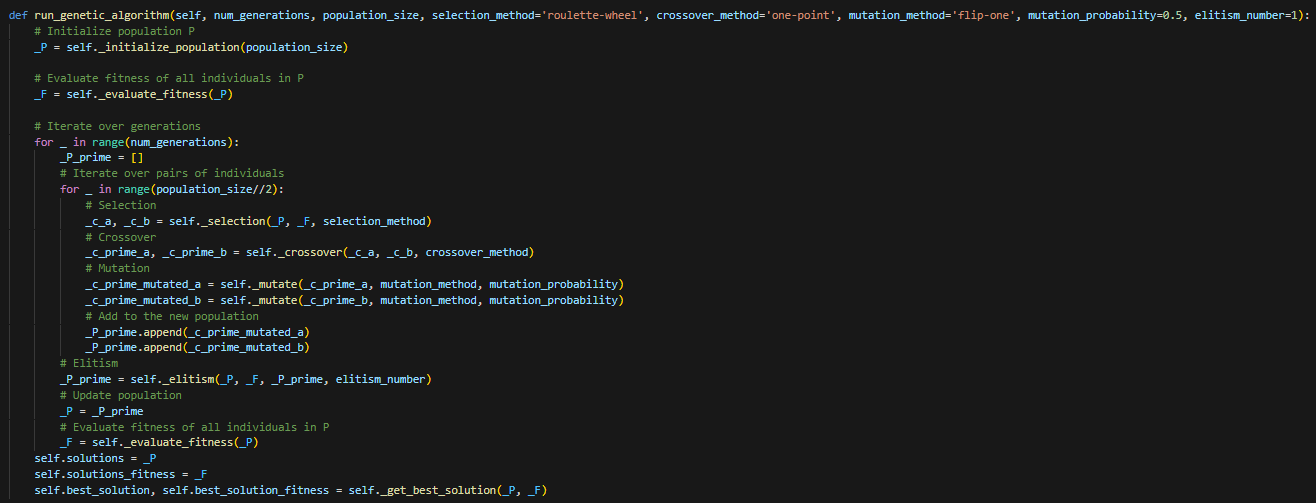
\includegraphics[width=\textwidth]{media/genetic_algorithm.png}
    \caption{Python code of the main genetic algorithm implementation}
    \label{fig:image_1}
\end{figure}

\subsection{Convert to chromosomes}

As mentioned before a chromosome is represented by a sequence of 0s and 1s such \(c \in \{0, 1\}^{n_{machines}}\). To get this result the format used 
has been (job\_index, operation\_index), the previous list is flattened \eqref{equation_5}.

\begin{equation}
    (i, j) \mid i \in \{0, 1, \dots, n_{jobs}-1\}, \, j \in \{0, 1, \dots, n_{machines}-1\}
    \label{equation_5}
\end{equation}

\newpage

The previous example looks as it follows after the transformation.

\[
\begin{aligned}
&\{(0, 0), (0, 1), \dots, (0, 9), \\
&\ (1, 0), (1, 1), \dots, (9, 9)\}
\end{aligned}
\]

This transformation is done by iterating over all the elements and saving their indexes in a tuple.

\begin{figure}[H]
    \centering
    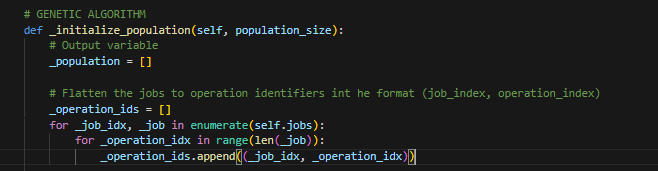
\includegraphics[width=\textwidth]{media/chromosomes_creation.png}
    \caption{Python code to convert the input data into chromosomes}
    \label{fig:image_8}
\end{figure}

\subsection{Creating the initial population}

To create the intial population it is necessary to transform the initial data into a chromosomes. The initial population is created randomly by creating
permutations. Basically, it is generated random permutations of operations while respecting job operation dependencies, ensuring that each operation is 
scheduled only after its preceding operation for the same job. This will always generate valid permutations.

\vspace{1em} The previous explained chromosome conversion and the creation of the initial population are done in the same method \_initialize\_population.

\begin{figure}[H]
    \centering
    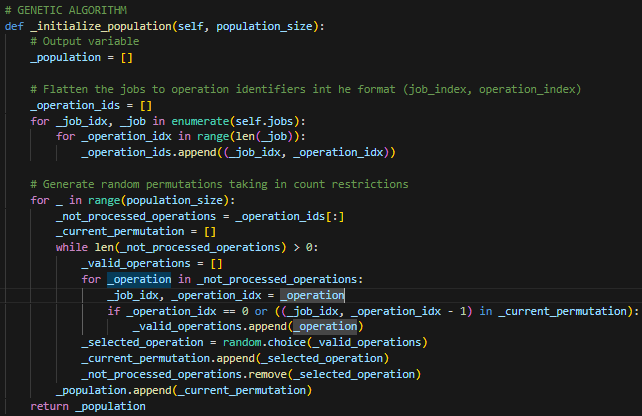
\includegraphics[width=0.8\textwidth]{media/population_init.png}
    \caption{Python code that genereates the initial populations}
    \label{fig:image_2}
\end{figure}


\subsection{Evaluate fitness}

Evaluating the fitness of the population is important to determine how well each solution satisfies the problem's constraints and to guide the selection of the best 
solutions for optimization. In this case, the fitness of each solution is evaluated by calculating the makespan, which is the total time required to complete all jobs. 
The evaluation ensures that each operation respects two key constraints: a machine cannot start a new operation until it is free, and a job cannot proceed to its next 
operation until the previous one is completed. These constraints are handled by calculating the earliest start time for each operation based on the availability of 
the machine and the job's completion. The fitness value is the maximum end time across all machines, representing the makespan.

\vspace{1em} To ensure that operations are scheduled according to the constraints, the function calculates the earliest possible start time for the operation. This is determined by taking 
the maximum of two values: the time when the machine becomes free (\_machine\_end\_times[\_machine]) and the time when the job becomes available (\_job\_end\_times[\_job\_idx]). 
The operation starts at the later of these two times to ensure both the machine and the job are ready.

\vspace{1em} Once the start time is determined, the end time of the operation is calculated by adding the processing time. The machine and job availability are then updated based on the 
operation’s end time. This step ensures that the machine and job schedules reflect the completion of this operation.

\vspace{1em} After all operations for the individual have been scheduled, the makespan is calculated as the maximum end time across all machines. This makespan represents the total time 
required to finish all operations in the schedule. The fitness of the individual is the value of this makespan, with a lower makespan indicating a better solution.

\begin{figure}[H]
    \centering
    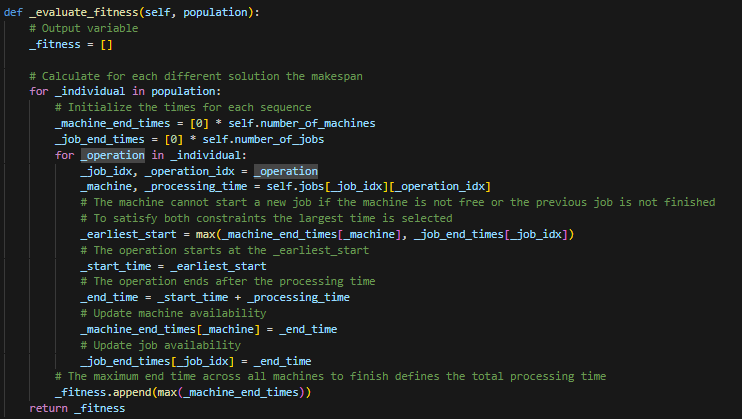
\includegraphics[width=\textwidth]{media/evaluate_fitness.png}
    \caption{Python code that calculates the fitness of the population}
    \label{fig:image_6}
\end{figure}

\subsection{Selection}

Selection ensures that better solutions have a higher chance of being passed on to the next generation. It drives the evolution towards optimal solutions by prioritizing 
individuals with higher fitness. The selection function chooses two individuals from the population based on their fitness, using either the tournament or roulette wheel method. 
It ensures that the most suitable candidates are selected for the next generation.

\vspace{1em} In the roulette wheel method, individuals are selected based on their fitness proportions. The higher an individual's fitness, the more likely it is to be selected. 
The selection is done by calculating the fitness percentage of each individual, followed by a random choice based on these probabilities.

\vspace{1em} In the tournament method, a subset of individuals is randomly selected from the population, and the fittest individual within this subset is chosen. This process is 
repeated to select two individuals, ensuring that the fittest candidates within the subset have a higher chance of selection.

\begin{figure}[H]
    \centering
    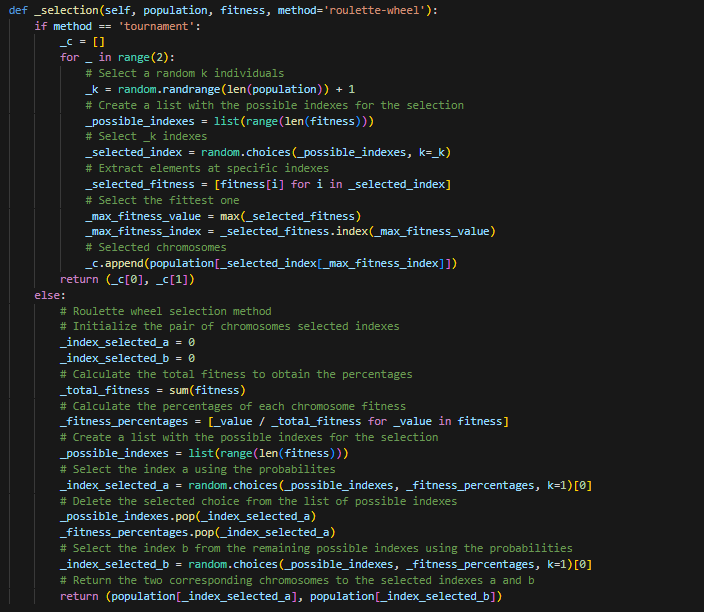
\includegraphics[width=\textwidth]{media/selection.png}
    \caption{Python code that implements the selection methods}
    \label{fig:image_7}
\end{figure}

\subsection{Crossover}

Crossovercombines the genetic material of two parents to produce offspring with characteristics from both. This helps explore new solutions and maintain genetic diversity 
in the population, driving the algorithm towards optimal results. The crossover function generates offspring by exchanging genetic material from two parent individuals. 
It allows different crossover methods, such as one-point and uniform crossover, to combine the parent solutions and create diverse offspring for the next generation.

\vspace{1em} In the uniform crossover method, each operation in the chromosomes is considered for swapping. With a 50\% probability, an operation from one parent is exchanged 
with the corresponding operation from the other parent. This method ensures that parts from both parents are mixed in the offspring.

\vspace{1em} In the one-point crossover method, a random crossover point is selected. The portion of the chromosome after this point is swapped between the two parents, 
generating two offspring that inherit parts of each parent before and after the selected point.

\begin{figure}[H]
    \centering
    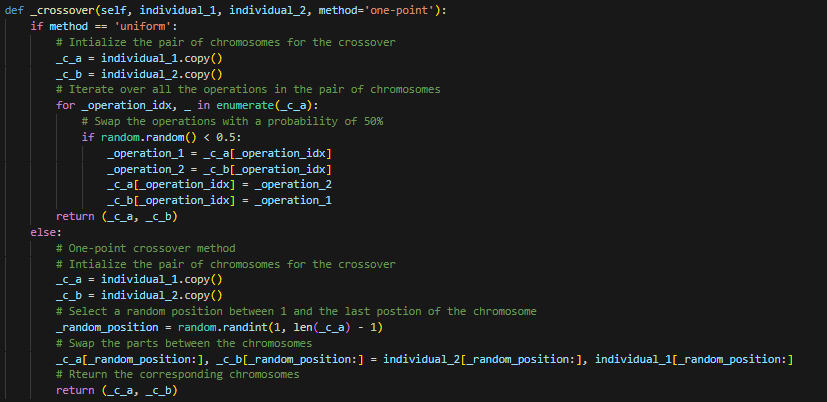
\includegraphics[width=\textwidth]{media/crossover.png}
    \caption{Python code that implements the crossover methods}
    \label{fig:image_9}
\end{figure}

\subsection{Mutation}

Mutation introduces random changes to individuals, helping to explore new solutions outside the current population's genetic pool. This helps prevent premature 
convergence and maintains diversity, ensuring the algorithm doesn't get stuck in local optima. The mutation function applies random changes to an individual’s chromosome. 
It provides different mutation methods, such as "flip-probabilistic" and "flip-one", to introduce variety by flipping parts of the chromosome and altering the solution.

\vspace{1em} In the flip-probabilistic mutation method, each operation in the chromosome has a certain probability of being flipped. If the random number is less than the probability, 
the operation's bits are negated, introducing variability and increasing genetic diversity.

\vspace{1em} In the flip-one mutation method, a random position in the chromosome is selected, and its value is flipped. This introduces a single mutation in the chromosome, altering 
the solution with minimal disruption while maintaining overall structure.

\begin{figure}[H]
    \centering
    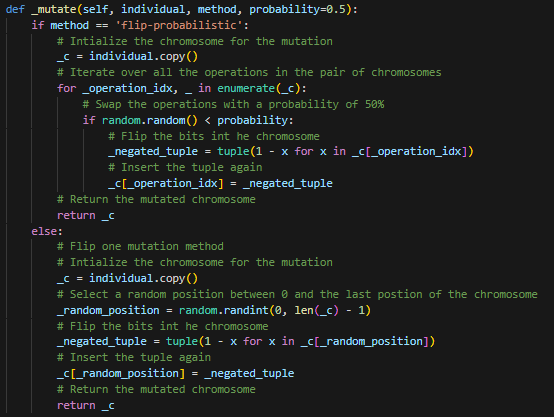
\includegraphics[width=\textwidth]{media/mutation.png}
    \caption{Python code that implements the crossover methods}
    \label{fig:image_10}
\end{figure}

\subsection{Elitism}

Elitism ensures the best solutions are carried forward to the next generation. Without elitism, there’s a risk of losing the best solution due to random 
crossover or mutation, thus preventing progress. This process helps to retain high-quality individuals and speeds up convergence. This implementation aims to preserve the 
best-performing individuals from one generation to the next. The elite individuals are selected from the current population based on their fitness, ensuring that they survive 
into the next generation. This increases the likelihood of finding better solutions over time.

\newpage

The function \_elitism takes two populations and their fitness values. It finds the number of individuals with the smallest fitness values (best solutions) from population\_1. 
These best individuals are added to population\_2, which is returned as the new population. The method uses heapq.nsmallest() to efficiently select the best individuals based on 
their fitness values.

\begin{figure}[H]
    \centering
    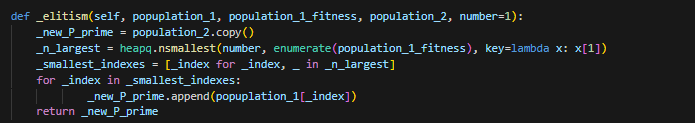
\includegraphics[width=\textwidth]{media/elitism.png}
    \caption{Python code that implements the elitism method}
    \label{fig:image_11}
\end{figure}

\subsection{Validate solution}

Validating ensures the generated solutions respect the problem's constraints. For the Job-Shop Scheduling Problem, a valid solution must follow job precedence and machine 
availability rules. If solutions violate these constraints, they become irrelevant, reducing the chances of finding a true optimal solution. By filtering out invalid solutions, 
the algorithm focuses on feasible solutions. After some mutation, crossover and selection steps some solutions could become invalid and those cannot be taken in count for the 
final selection of the fitest one. The \_validate\_solution function checks whether a given solution satisfies the constraints of the Job-Shop Scheduling Problem. It verifies the job precedence and ensures 
machines are available before processing operations. If any constraint is violated, it returns False. The \_get\_best\_solution function refines the population by removing invalid 
solutions and selects the best valid solution based on fitness. The filtered population is then used to track and update the best solution found.

\vspace{1em} The \_validate\_solution method iterates over each operation in a solution. For each operation, it checks if job precedence is maintained and if machines are available 
to process the operation without conflicts. If any of the constraints are violated, the solution is invalid, and the method returns False. Otherwise, it updates machine and job end 
times and returns True.

\vspace{1em}The \_get\_best\_solution function first filters out invalid solutions from the population using the \_validate\_solution method. It then identifies the best solution among 
the valid ones by selecting the one with the lowest fitness value. If no valid solutions remain, it returns a placeholder value [-1, -1] to indicate failure. The function ensures that 
only feasible solutions are considered.

\begin{figure}[H]
    \centering
    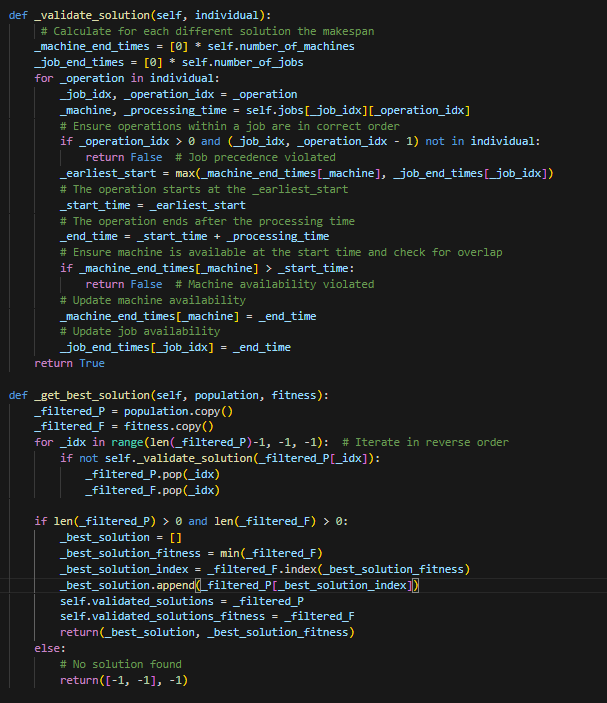
\includegraphics[width=\textwidth]{media/validate_solution.png}
    \caption{Python code that implements the validation methods}
    \label{fig:image_12}
\end{figure}

\newpage

\section{Results}

Some validations have been done using datasets from https://people.brunel.ac.uk/~mastjjb/jeb/orlib/files/jobshop1.txt. 

\subsection{Instance ft06 - Fisher and Thompson 6x6 instance}

This instance has 6 machines and 6 jobs. Tg

\begin{table}[H]
    \centering
    \resizebox{\textwidth}{!}{
    \begin{tabular}{|c|c|c|c|c|c|}
    \hline
    \textbf{Number of Generations} & \textbf{Initial Population Size} & \textbf{Selection Method} & \textbf{Crossover Method} & \textbf{Mutation Method} & \textbf{Fitness} \\ \hline
    20                             & 100                              & Roulette wheel            & One-point                 & Bit-Flip                 & 56             \\ \hline
    20                             & 100                              & Tournament                & One-point                 & Bit-Flip                 & 68             \\ \hline
    20                             & 100                              & Roulette wheel            & Uniform                   & Bit-Flip                 & 60             \\ \hline
    20                             & 100                              & Tournament                & Uniform                   & Bit-Flip                 & 69             \\ \hline
    20                             & 100                              & Roulette wheel            & One-point                 & Probabilistic (0.1)      & 68             \\ \hline
    20                             & 100                              & Tournament                & One-point                 & Probabilistic (0.1)      & 69             \\ \hline
    \end{tabular}
    }
    \caption{Results for instance ft06 with different parameter combinations}
    \label{tab:table_2}
\end{table}

The last test (tournament, one-point and probabilistic (0.1)) has been represented in a gnatt chart for better understanding of the solutions.

\begin{figure}[H]
    \centering
    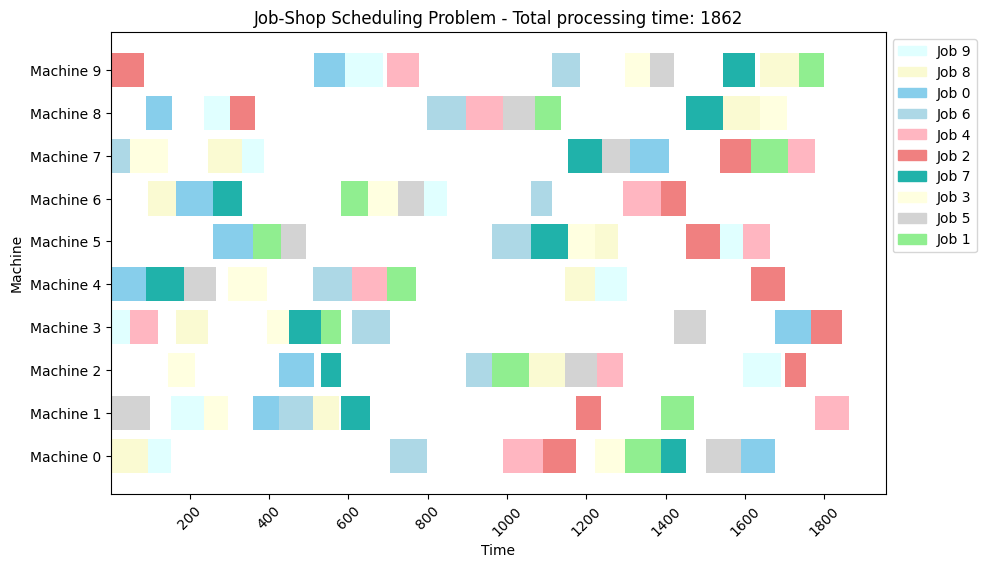
\includegraphics[width=\textwidth]{media/results_abz5.png}
    \caption{Gnatt chart of the last entry in the table \ref{table_2}}
    \label{fig:image_13}
\end{figure}

\subsection{Instance abz5 - Adams, Balas, and Zawack 10x10 instance}

This instance has 10 machines and 10 jobs.

\begin{table}[H]
    \centering
    \resizebox{\textwidth}{!}{
    \begin{tabular}{|c|c|c|c|c|c|}
    \hline
    \textbf{Number of Generations} & \textbf{Initial Population Size} & \textbf{Selection Method} & \textbf{Crossover Method} & \textbf{Mutation Method} & \textbf{Fitness} \\ \hline
    20                             & 100                              & Roulette wheel            & One-point                 & Bit-Flip                 & 1495             \\ \hline
    20                             & 100                              & Tournament                & One-point                 & Bit-Flip                 & 1796             \\ \hline
    20                             & 100                              & Roulette wheel            & Uniform                   & Bit-Flip                 & 1699             \\ \hline
    20                             & 100                              & Tournament                & Uniform                   & Bit-Flip                 & 1773             \\ \hline
    20                             & 100                              & Roulette wheel            & One-point                 & Probabilistic (0.1)      & 1913             \\ \hline
    20                             & 100                              & Tournament                & One-point                 & Probabilistic (0.1)      & 1862             \\ \hline
    \end{tabular}
    }
    \caption{Results for instance la36 with different parameters}
    \label{tab:table_1}
\end{table}

The last test (tournament, one-point and probabilistic (0.1)) has been represented in a gnatt chart for better understanding of the solutions.

\begin{figure}[H]
    \centering
    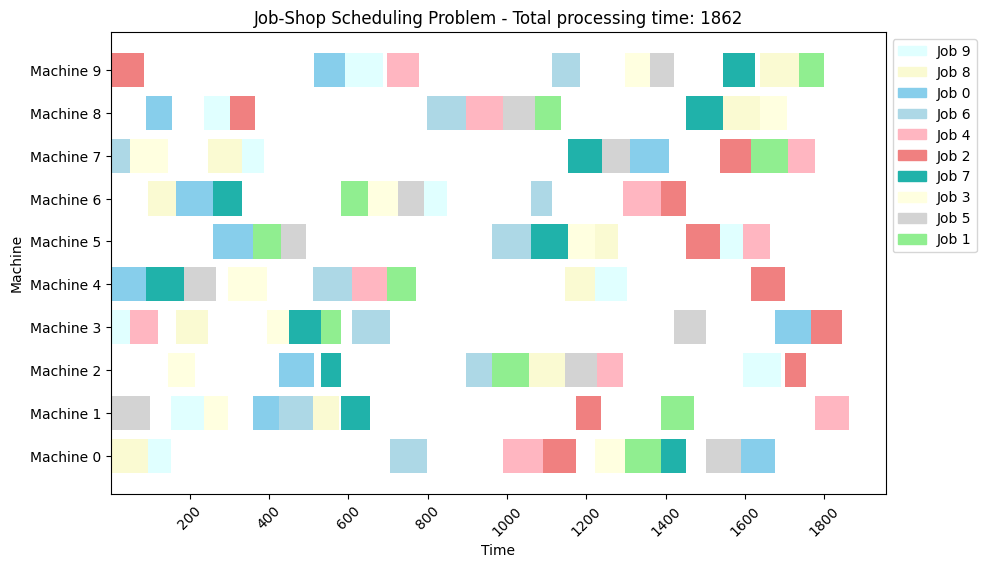
\includegraphics[width=\textwidth]{media/results_abz5.png}
    \caption{Gnatt chart of the last entry in the table \ref{table_1}}
    \label{fig:image_14}
\end{figure}

\subsection{Instance la36 - Lawrence 15x15 instance}

This instance has 15 machines and 15 jobs.
\begin{table}[H]
    \centering
    \resizebox{\textwidth}{!}{
    \begin{tabular}{|c|c|c|c|c|c|}
    \hline
    \textbf{Number of Generations} & \textbf{Initial Population Size} & \textbf{Selection Method} & \textbf{Crossover Method} & \textbf{Mutation Method} & \textbf{Fitness} \\ \hline
    20                             & 100                              & Roulette wheel            & One-point                 & Bit-Flip                 & 2042             \\ \hline
    20                             & 100                              & Tournament                & One-point                 & Bit-Flip                 & 2420             \\ \hline
    20                             & 100                              & Roulette wheel            & Uniform                   & Bit-Flip                 & 2387             \\ \hline
    20                             & 100                              & Tournament                & Uniform                   & Bit-Flip                 & 2287             \\ \hline
    20                             & 100                              & Roulette wheel            & One-point                 & Probabilistic (0.1)      & 2227             \\ \hline
    20                             & 100                              & Tournament                & One-point                 & Probabilistic (0.1)      & 2281             \\ \hline
    \end{tabular}
    }
    \caption{Results for instance la36 with different parameters}
    \label{tab:table_3}
\end{table}


The last test (tournament, one-point and probabilistic (0.1)) has been represented in a gnatt chart for better understanding of the solutions.

\begin{figure}[H]
    \centering
    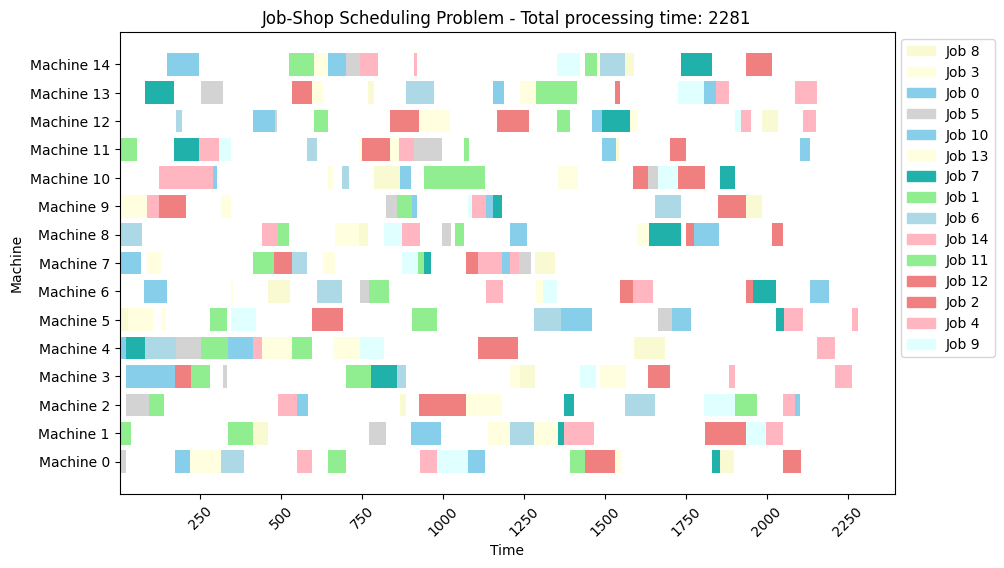
\includegraphics[width=\textwidth]{media/results_la36.png}
    \caption{Gnatt chart of the last entry in the table \ref{table_3}}
    \label{fig:image_15}
\end{figure}


\subsection{Minimum travel tiempo across generations}

After carrying several tests, it became apparent that many of the solutions generated across multiple generations were either identical or extremely similar to the initial solutions. 
This phenomenon primarily stems from the fact that the crossover and mutation operations frequently produced invalid solutions, which were subsequently discarded during the validation 
phase. The high number of invalid solutions can be attributed to the nature of these genetic operations, which often do not respect the problem constraints, such as job precedence or 
machine availability, thus leading to infeasible solutions.

\vspace{1em} The persistent generation of invalid solutions indicates a need for more effective genetic operators—specifically, crossover and mutation methods better tailored to the 
constraints and characteristics of the Job Shop Scheduling Problem (JSSP). A key challenge here is ensuring that the crossover and mutation processes generate solutions that remain 
valid and feasible throughout the evolutionary process.

\begin{figure}[H]
    \centering
    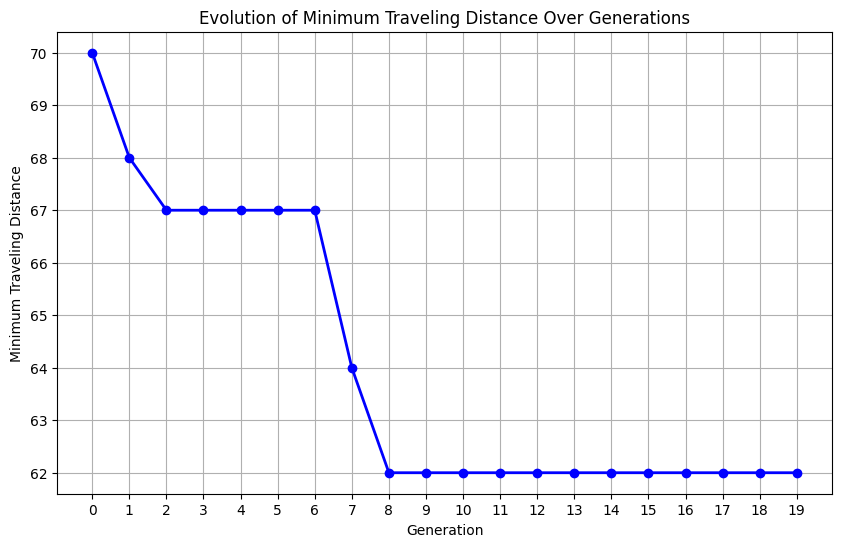
\includegraphics[width=0.8\textwidth]{media/minimum_travel_distance_ft06.png}
    \caption{Minimum travel distance for a ft06 instance execution}
    \label{fig:image_16}
\end{figure}

\vspace{1em} To address this issue, selecting more appropriate crossover and mutation methods should be explored. For example, order-based crossover methods, like OX (Order Crossover) 
or PMX (Partially Matched Crossover), have been shown to perform well in combinatorial problems, especially those involving ordered sets like job schedules. These methods are designed 
to preserve the relative order of genes in the offspring, which helps maintain the feasibility of the solution. It would be a possibility to explore this ways.

\begin{figure}[H]
    \centering
    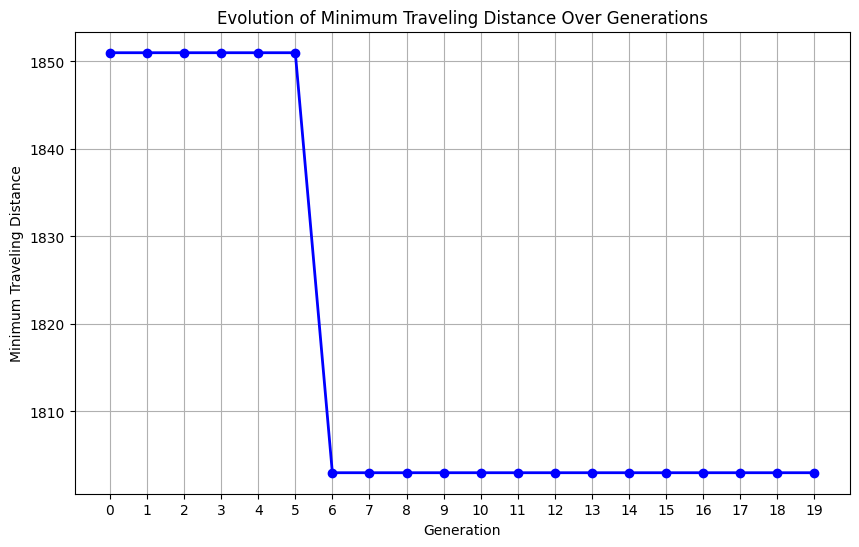
\includegraphics[width=0.8\textwidth]{media/minimum_travel_distance_abz5.png}
    \caption{Minimum travel distance for a abz5 instance execution}
    \label{fig:image_17}
\end{figure}

\vspace{1em} In terms of mutation, swap mutation is another useful technique for job-shop problems, where two jobs are swapped within a machine or between machines. This type of mutation e
nsures that the job schedule remains valid by keeping the sequence intact while introducing variability. Alternatively, insertion-based mutation, where a job is moved to a different position 
in the schedule, can help explore the search space more efficiently.

\begin{figure}[H]
    \centering
    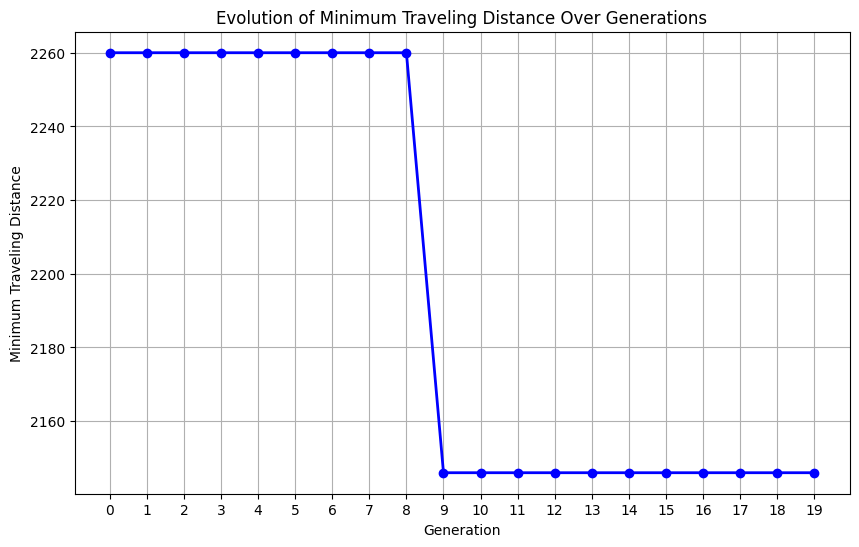
\includegraphics[width=0.8\textwidth]{media/minimum_travel_distance_la36.png}
    \caption{Minimum travel distance for a la36 instance execution}
    \label{fig:image_18}
\end{figure}

\vspace{1em} In conclusion, the frequent generation of invalid solutions in the current approach emphasizes the importance of selecting crossover and mutation methods that are specifically 
designed to maintain the feasibility of the solution. By incorporating these more sophisticated genetic operators, probably we will get better results.

\section{Conclusion}

Genetic algorithms (GA) show potential for solving the Job Shop Scheduling Problem. They can explore large search spaces and find good solutions quickly. However, the crossover and mutation 
methods must be carefully chosen to produce valid solutions. Adjusting the population size and fine-tuning operators can improve performance. Despite challenges like premature convergence, 
experimenting with different GA variations may lead to better results.

\subsection{Further steps}

The genetic algorithm (GA) showed that many solutions in later generations were similar or the same as the initial solutions. This happened because the crossover and mutation methods often 
produced invalid solutions. These solutions were discarded during validation. Validation is crucial in filtering out invalid solutions. However, this process shows the need for better solution generation methods. 
The current crossover and mutation strategies often require discarding too many solutions. In other words, the crossover and mutation methods used need to be more suited to the problem. They should generate more 
valid solutions. Due to time restriction I could not explore this posibilities.

\newpage

\begin{thebibliography}{11}

\bibitem{WikipediaGA}
Wikipedia contributors, \textit{Genetic algorithm}, Wikipedia, The Free Encyclopedia, 
Available at \url{https://en.wikipedia.org/wiki/Genetic\_algorithm}, 
accessed January 18, 2025.

\bibitem{WikipediaEC}
Wikipedia contributors, \textit{Evolutionary computation}, Wikipedia, The Free Encyclopedia, 
Available at \url{https://en.wikipedia.org/wiki/Evolutionary_computation}, 
accessed January 18, 2025.

\bibitem{WikipediaJSSP}
Wikipedia contributors, \textit{Job-shop scheduling}, Wikipedia, The Free Encyclopedia, 
Available at \url{https://en.wikipedia.org/wiki/Job-shop_scheduling}, 
accessed January 19, 2025.

\bibitem{WikipediaSelection}
Wikipedia contributors, \textit{Selection (evolutionary algorithm)}, Wikipedia, The Free Encyclopedia, 
Available at \url{https://en.wikipedia.org/wiki/Selection_(evolutionary_algorithm)}, 
accessed January 19, 2025.

\bibitem{WikipediaCrossover}
Wikipedia contributors, \textit{Crossover (evolutionary algorithm)}, Wikipedia, The Free Encyclopedia, 
Available at \url{https://en.wikipedia.org/wiki/Crossover_(evolutionary_algorithm)}, 
accessed January 19, 2025.

\bibitem{WikipediaMutation}
Wikipedia contributors, \textit{Mutation (evolutionary algorithm)}, Wikipedia, The Free Encyclopedia, 
Available at \url{https://en.wikipedia.org/wiki/Mutation_(evolutionary_algorithm)}, 
accessed January 19, 2025.

\end{thebibliography}

\end{document}
